\documentclass[tikz,border=5pt]{standalone}
\usepackage{tikz}
\usepackage{amsmath}
\begin{document}

\begin{figure}[H]
\begin{center}
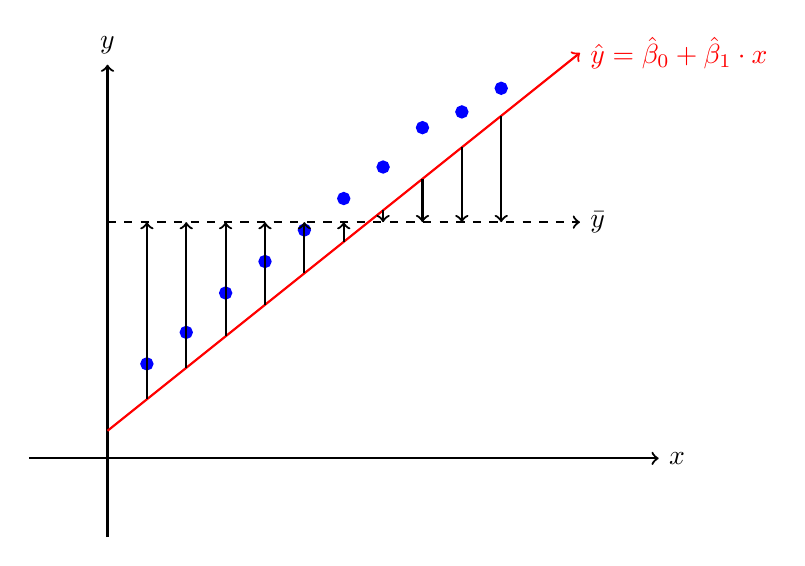
\begin{tikzpicture}[->, thick]
  \draw[->] (-1,0) -- (7,0) node[right] {$x$};
  \draw[->] (0,-1) -- (0,5) node[above] {$y$};
  \filldraw[blue] (0.5, 1.2) circle (2pt);
  \filldraw[blue] (1.5, 2.1) circle (2pt);
  \filldraw[blue] (1, 1.6) circle (2pt);
  \filldraw[blue] (2, 2.5) circle (2pt);
  \filldraw[blue] (2.5, 2.9) circle (2pt);
  \filldraw[blue] (3, 3.3) circle (2pt);
  \filldraw[blue] (3.5, 3.7) circle (2pt);
  \filldraw[blue] (4, 4.2) circle (2pt);
  \filldraw[blue] (4.5, 4.4) circle (2pt);
  \filldraw[blue] (5, 4.7) circle (2pt);
  \draw[red, thick, domain=0:6] plot (\x, {0.8*\x + 0.35}) node[right] {$\hat{y} = \hat{\beta}_0 + \hat{\beta}_1 \cdot x$};
  \draw[dashed] (0,3) -- (6,3) node[right] {$\bar{y}$};
  \foreach \x in {0.5, 1, 1.5, 2, 2.5, 3, 3.5, 4, 4.5, 5} {
    \draw[black] (\x, {0.8*\x + 0.35}) -- (\x, 3);
  }
\end{tikzpicture}
\end{center}
\caption{An illustration of simple linear regression. The blue points represent monthly height measurements with added variability. The red line is the fitted simple linear regression model. The dashed line shows the mean of the dependent variable, $\bar{y}$, and the solid black lines illustrate the deviation of the model's predictions from this mean.}
\end{figure}

\end{document}